\subsection{Introduction}

When we talked about derivatives, we relied on the idea of limits - something that could "zoom in" to a point that was not necessarily defined - but we left the actual mechanics of them rather sketchily laid out.

Let's think about what we want a limit to do. Imagine we have the function

\begin{equation*}
    f(x) = \frac{(3x+1)(x-1)}{(x-1)}
\end{equation*}

When we graph it, we get a hole at the point where $x=1$ - the function is undefined there. But imagine if we look at the points really close to that hole on either side - where $x=.99$ or $x = 1.01$. What do those values approach?

\begin{center}
    \begin{tabular}{c|c|c|c}
       $x < 1$  &  $y$ & $x > 1$ & $y$\\
       \hline
        $0.99$ & $3.97$ & $1.01$&$4.03$ \\
        $.999$ & $3.997$ & $1.001$&$4.003$ \\
        $.9999$ & $3.9997$ & $1.0001$& $4.0003$
    \end{tabular}
\end{center}

We want our definition of a limit, when given this function and told to approach $1$, to produce an outcome of $4$.

We also want our limit contraption to spit out the right thing if there {\it isn't} a hole: if we find the limit as $x$ tends to $1$ of $y=x$, our limit should result in $1$. In other words, our definition of a limit shouldn't do something crazy when normal inputs, else it isn't the definition we want.

\subsection{Formal definition}

Now that we know what our definition of limits needs to entail

\subsection{Solving limits}
\subsubsection{Using the definition}



\subsubsection{Proof-free methods}

One does not need to use an epsilon-delta proof every time. Much like with the derivative, you can use the full definition, or you can just use the rules that pop out of the definition (or in this case, tricks for rearranging things) to solve the problem more easily.

The first type of limit you could call an "easy" limit. 
All you have to do is plug in the number you are approaching for your variable, because the function doesn't violate any rules like we described above. 
So for example, if you have the limit

\begin{equation*}
    \lim\limits_{x\rightarrow 1} x
\end{equation*}

You would just get 1. 
Other limits require a little more work. For instance, say we have
\begin{equation*}
    \lim\limits_{x\rightarrow -3}\frac{x^2-x-12}{x+3}
\end{equation*}
We can clearly see that if we just plug it in, there will be a zero in the denominator. 
Instead, we can try messing around with the expression using tools like factoring or rationalizing the denominator. 
In this particular case, the expression in the numerator is very easy to factor:
\begin{equation*}
    \lim\limits_{x\rightarrow -3}\frac{(x+3)(x-4)}{x+3}
\end{equation*}
This then leaves us with
\begin{equation*}
    \lim\limits_{x\rightarrow -3}x-4
\end{equation*}
The limit is now one of our "easy" limits, so we can simply plug in $-3$. The answer is $-7$.

Now we have our final type of limit, the "$\frac{\text{not zero}}{0}$" limit. 
This type of limit is a bit different from the other two types of limits. As an example, let's say we are trying to solve the problem
\begin{equation*}
    \lim\limits_{x\rightarrow 0}\frac{1}{x}
\end{equation*}
To solve this, we must first solve
\begin{equation*}
    \lim\limits_{x\rightarrow 0^+}\frac{1}{x}
\end{equation*}
and
\begin{equation*}
    \lim\limits_{x\rightarrow 0^-}\frac{1}{x}
\end{equation*}
Looking at the second problem first, the $+$ sign means it is a right limit - that is, we are approaching zero from the left. Let's say we have a number line like the one below.

\begin{figure}[H]
\centering
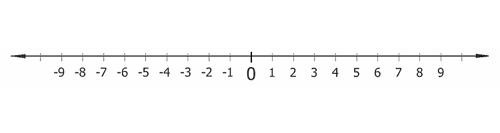
\includegraphics[scale=0.5]{numberline.jpg}
\end{figure}

To approach from the right means that $x$ will be represented by tiny positive numbers, like $0.00001$ and $0.0000001$, that get closer and closer to $0$. 

Thus, the answer to this particular limit will be whatever $\frac{1}{\text{really small positive number}}$ is. 
For instance, if we have $\frac{1}{0.00001}$ we get $100000$; if we have something closer to zero, like $\frac{1}{0.0000001}$ we get $10000000$. 
In other words, we are approaching infinity, so $+\infty$ is our solution.

If we look at the first problem, this time, we are approaching zero from the left, so we are dividing by negative numbers. (It's very easy to check your work for most limits on a calculator by plugging in numbers and seeing what it approaches.) It turns out that this approaches $-\infty$. 

Now, to solve the original limit. 
If we take the two limits we split the original into and their answer is the same, the first limit has a solution, but in our case the second two limits had different solutions, meaning there is no answer. What we're doing here is seeing if there's a big jump between the left and the right or not.

\subsubsection{L'H\^{o}pital's Rule}

Sometimes we get limits that we cannot manipulate, and when you plug in the limit it turns into something nasty and unworkable like $\frac{0}{0}$ or $\pm\frac{\infty}{\infty}$.

You'll notice in the past that when we've taken the derivative of functions they tend to become less disgusting - powers get reduced, constants get thrown out, etc. Perhaps you see where this is going.

talk about geometric approach? slopes match up - but only in certain cases, why only in certain cases